%%%%%%%%%%%%%%%%%%%%%%%%%%%%%%%%%%%%%%%%%%%%%%%%%%%%%%%%%%%%%%%%%%%%%%
% LaTeX Example: Project Report
%
% Source: http://www.howtotex.com
%
% Feel free to distribute this example, but please keep the referral
% to howtotex.com
% Date: March 2011 
% 
%%%%%%%%%%%%%%%%%%%%%%%%%%%%%%%%%%%%%%%%%%%%%%%%%%%%%%%%%%%%%%%%%%%%%%
% How to use writeLaTeX: 
%
% You edit the source code here on the left, and the preview on the
% right shows you the result within a few seconds.
%
% Bookmark this page and share the URL with your co-authors. They can
% edit at the same time!
%
% You can upload figures, bibliographies, custom classes and
% styles using the files menu.
%
% If you're new to LaTeX, the wikibook is a great place to start:
% http://en.wikibooks.org/wiki/LaTeX
%
%%%%%%%%%%%%%%%%%%%%%%%%%%%%%%%%%%%%%%%%%%%%%%%%%%%%%%%%%%%%%%%%%%%%%%
% Edit the title below to update the display in My Documents
%\title{Project Report}
%
%%% Preamble
\documentclass[paper=a4, fontsize=11pt]{scrartcl}
\usepackage[T1]{fontenc}
\usepackage[utf8]{inputenc}
\usepackage{amsmath,amsfonts,amsthm} % Math packages
\usepackage[pdftex]{graphicx}	
\usepackage{url}
\usepackage[skip=2pt]{caption} % example skip set to 2pt
\usepackage[croatian]{babel}
\usepackage{listings}
\usepackage{enumitem}

%%% Custom sectioning
\usepackage{sectsty}
\allsectionsfont{\centering \normalfont\scshape}


%%% Custom headers/footers (fancyhdr package)
\usepackage{fancyhdr}
\pagestyle{fancyplain}
\fancyhead{}											% No page header
\fancyfoot[L]{}											% Empty 
\fancyfoot[C]{}											% Empty
\fancyfoot[R]{\thepage}									% Pagenumbering
\renewcommand{\headrulewidth}{0pt}			% Remove header underlines
\renewcommand{\footrulewidth}{0pt}				% Remove footer underlines
\setlength{\headheight}{13.6pt}


%%% Equation and float numbering
\numberwithin{equation}{section}		% Equationnumbering: section.eq#
\numberwithin{figure}{section}			% Figurenumbering: section.fig#
\numberwithin{table}{section}				% Tablenumbering: section.tab#

%%% Maketitle metadata
\newcommand{\horrule}[1]{\rule{\linewidth}{#1}} 	% Horizontal rule

\title{
		%\vspace{-1in} 	
		\usefont{OT1}{bch}{b}{n}
		\normalfont \normalsize \textsc{Fakultet Elektrotehnike i Računarstva} \\ [25pt]
		\horrule{0.5pt} \\[0.4cm]
		\huge 4. Laboratorijska vježba - ROVKP \\
		\horrule{2pt} \\[0.5cm]
}
\author{
		\normalfont 								\normalsize
        Vinko Kolobara\\[-3pt]		\normalsize
        \today
}
\date{}


%%% Begin document
\begin{document}
\maketitle

\section{Zadatak: Obrada podataka programskim okvirom Apache Spark}
1. Koliko je ženskih osoba umro u lipnju kroz čitav period?\\
$100654$\\

2. Koji dan u tjednu je umrlo najviše muških osoba starijih od 50 godina?\\
Četvrtak.\\

3. Koliko osoba je bilo podvrgnuto obdukciji nakon smrti?\\
$203681$\\

4. Kakvo je kretanje broja umrlih muškaraca u dobi između 45 i 65 godina po mjesecima ? Rezultat je (sortirana) lista tipa Pair2 (ključ je redni broj mjeseca, a vrijednost je broj umrlih muškaraca)\\

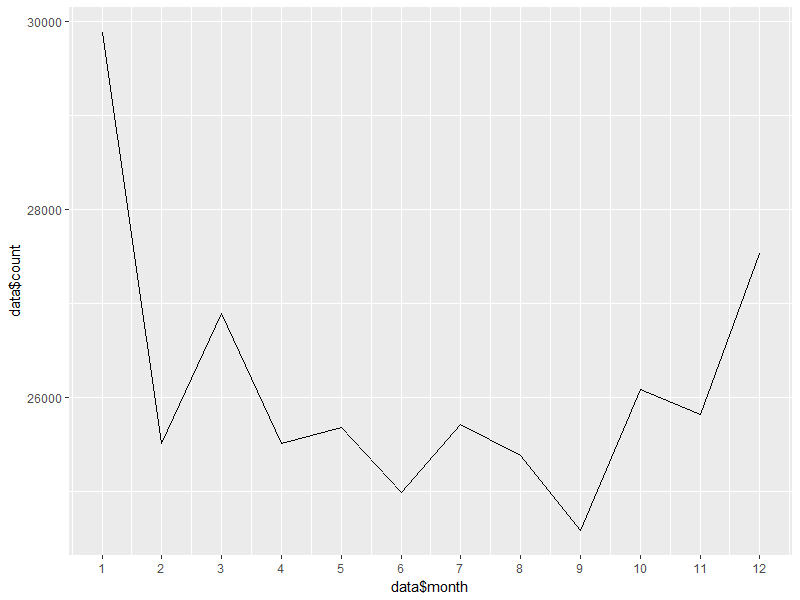
\includegraphics[width=\textwidth]{deadMales.png}

5. Kakvo je kretanje postotka umrlih oženjenih muškaraca u dobi između 45 i 65 godina po mjesecima? Rezultat je (sortiran) skup tipa Pair2 (ključ je redni broj mjeseca, a vrijednost je postotak). \\

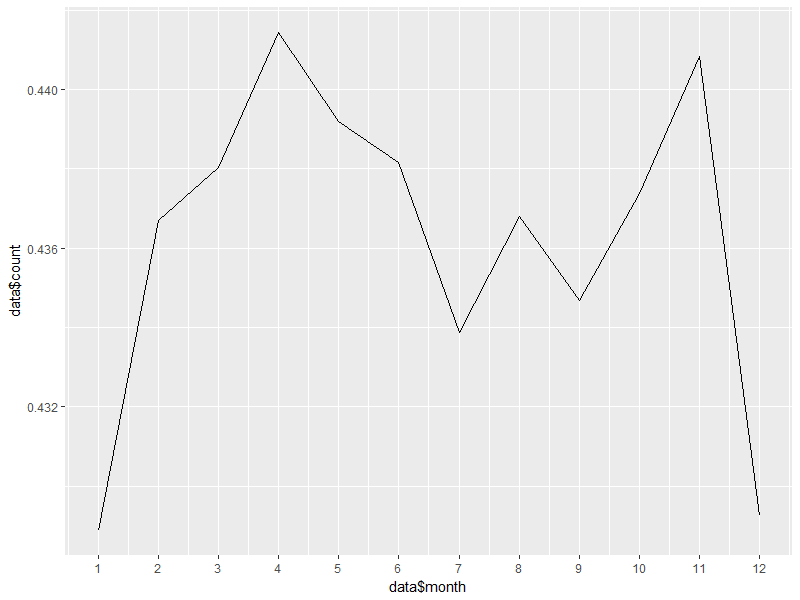
\includegraphics[width=\textwidth]{marriedDeadMales.png}

6. Koji je ukupni broj umrlih u nesreći (kod 1) u cjelokupnom periodu?\\
$132684$

7. Koliki je broj različitih godina starosti umrlih osoba koji se pojavljuju u zapisima?\\
$117$

\pagebreak

\end{document}